\documentclass[sigplan,10pt,anonymous,review]{acmart}

\settopmatter{printfolios=true,printccs=false,printacmref=false}
\renewcommand\footnotetextcopyrightpermission[1]{}
\pagestyle{plain}

\usepackage{booktabs}
\usepackage{graphicx}
\usepackage{multirow}
\usepackage{subcaption}
\usepackage{xspace}
\usepackage{enumitem}
\usepackage{tikz}
\usetikzlibrary{arrows.meta,positioning,fit,calc,shapes.geometric}
\graphicspath{{figures/}{paper/figures/}}
\makeatletter
\def\input@path{{./}{paper/}}
\makeatother

\newcommand{\system}{CodeMAS\xspace}
\newcommand{\kvcomm}{KVCOMM\xspace}
\newcommand{\exactgate}{\texttt{exact\_code\_content\_signature}\xspace}
\newcommand{\prefetchhint}{\texttt{codebase\_prefetch\_hints}\xspace}

\title{Template-Guided Code-Base Segment Reuse for Multi-Agent Software Engineering}
\author{Anonymous Authors}
\affiliation{\institution{Anonymous Institution}}

\begin{document}

\begin{abstract}
Multi-agent systems for software engineering increasingly decompose a task into planner, implementer, debugger, and reviewer roles.
These agents often share a large repository context, but conventional prefix caching is poorly matched to this access pattern: the repeated content is not only at the prompt prefix, and the same code base may appear after different role-specific instructions and intermediate context.
This paper presents \system, a template-guided serving stack for coding multi-agent systems.
\system builds on prior workflow-aware cache scheduling and cross-context KV reuse, including KVFlow and \kvcomm, but focuses on the software-engineering case where the reusable object is an exact repository code segment.
\system contributes three code-specific mechanisms.
First, workflow templates expose future code-base access patterns across agents.
Second, a coding-aware hint schema propagates code-base identifiers, content signatures, priorities, and downstream consumers to the serving engine without treating hints as correctness evidence.
Third, an exact-content reuse policy uses AST and anchor metadata only to locate candidate code spans, requires an exact content signature match before reuse, and applies a RoPE delta transform when cached KV tensors are consumed at different prompt positions.

On SWE-bench Verified code-base-content workloads, \system identifies 58.8M reusable code tokens across 500 repo-level cases.
In controlled safety tests, the exact-content gate has zero false accepts, while AST-only and span-only gates accept semantically changed code.
In numerical ablations, correct RoPE delta alignment reaches 0.999 mean K cosine, 0.0147 next-token KL divergence, and 96.9\% top-1 token agreement.
On a 30-case local SWE-bench pass@1 comparison with Qwen2.5-7B-Instruct, exact-content segment reuse preserves the lossless baseline within one solved case while increasing average cached tokens from 1253 to 2190 and reducing generation latency from 2052 ms to 1729 ms.
These results suggest that coding-aware templates can turn repository repetition into safe serving-time KV reuse without allowing approximate or AST-only code substitution.
\end{abstract}

\begin{CCSXML}
<ccs2012>
 <concept>
  <concept_id>10010520.10010521.10010542</concept_id>
  <concept_desc>Computer systems organization~Distributed architectures</concept_desc>
  <concept_significance>300</concept_significance>
 </concept>
 <concept>
  <concept_id>10011007.10010940.10010941.10010949</concept_id>
  <concept_desc>Software and its engineering~Software testing and debugging</concept_desc>
  <concept_significance>300</concept_significance>
 </concept>
</ccs2012>
\end{CCSXML}
\ccsdesc[300]{Computer systems organization~Distributed architectures}
\ccsdesc[300]{Software and its engineering~Software testing and debugging}
\keywords{LLM serving, KV cache, multi-agent systems, software engineering agents, code generation}

\maketitle

\section{Introduction}

Coding multi-agent systems (MAS) are a natural fit for software engineering tasks~\cite{swebench,multiagent2025,llmagents2024}.
A planner can inspect the issue and decide which files matter; an implementer can edit the code; a debugger can reason over failures; a reviewer can verify the final patch.
However, this decomposition creates a serving-system mismatch.
Each agent typically receives a different instruction prefix and different intermediate context, yet many agents repeatedly read the same repository files.
The shared content is therefore a large code-base segment embedded at different prompt positions, rather than a simple common prefix.

Modern LLM serving systems reduce prefill and decode cost through paged KV memory, structured program execution, semantic variables, workflow-aware cache scheduling, and KV-centric agent serving~\cite{kwon2023vllm,zheng2023sglang,parrot2024,kvflow2025,tokencake2025}.
However, existing prefix-cache mechanisms accelerate exact shared prefixes.
They do not directly address repeated middle or suffix spans.
A serving engine may observe that two prompts both contain the same large code file, but the cached KV tensors for that file were produced at different RoPE positions.
Naively reusing them can perturb attention behavior; using syntax or anchor similarity as a gate can be unsafe because the same AST shape or function name can hide behavior-changing edits.

This paper argues that coding MAS creates a structured opportunity for safe lossy KV reuse.
The word ``lossy'' in this work has a narrow meaning: KV tensors are reused across different prompt positions after RoPE delta alignment.
It does not mean that different or approximate code content may be reused.
Our safety rule is strict: AST, anchors, file paths, and span overlap are locators only; reuse is allowed only when the normalized code content signature is exactly identical.

We present \system, a template-guided serving stack for coding MAS.
\system connects three layers.
At the template layer, a workflow describes how Planner, Implementer, Debugger, and Reviewer agents will consume code-base segments.
At the scheduling layer, these templates emit coding-aware hints, including \prefetchhint, so a KVFlow-style engine can prepare code-base KV before a later agent needs it.
At the reuse layer, the prototype adapts cross-context KV reuse ideas from \kvcomm to code segments: it locates candidate spans, enforces \exactgate, and rotates cached K/V tensors using the RoPE position delta.
This framing borrows the original AgentTemplateKV insight that agent DAGs, roles, and tool edges are serving-time signals, but specializes it to repo-level coding workloads where large exact code files dominate the reusable context.

The contributions are:
\begin{itemize}[leftmargin=*]
\item We identify code-base repetition as a distinct cache-reuse pattern in coding MAS: large exact code segments recur across agents but not necessarily at prompt prefixes.
\item We design a template-derived code-base hint schema that exposes future code-base use through \prefetchhint while preserving a strict separation between scheduling hints and reuse safety gates.
\item We implement a code-specific exact-content reuse policy on top of an SGLang/KVFlow-style prototype, combining candidate localization, content-signature gating, and RoPE delta alignment without claiming KVFlow or \kvcomm themselves as new contributions.
\item We evaluate \system on SWE-bench Verified code-base workloads, controlled ablations, repo-level reuse experiments, and local pass@1 tests, showing zero false accepts for the full gate, near-lossless logit behavior, and cached-token/latency gains with small lossless-vs-lossy accuracy delta.
\end{itemize}

\section{Motivation}

\subsection{Repository Context Repeats Across Agents}

In a coding MAS workflow, agents have different roles but often consult the same code base.
For example, a Planner may receive a repository summary and several large files to decide a repair strategy.
An Implementer later receives the issue, the plan, and two of the same files.
A Debugger may receive test output plus one of the same files.
The repeated code is exact, but its prompt position changes because each agent has a different prefix and context.
This is the common case rather than an artifact of a particular prompt template: role instructions, chain-of-thought summaries, test output, and tool results are usually prepended before the code that a later agent must inspect.
As a result, the expensive tokens are stable as repository content but unstable as prefix positions.

This pattern is not rare in repo-level tasks.
Our 500-case SWE-bench Verified code-base-content manifest contains 1500 large Python file segments, 5.97M source lines, and an estimated 58.8M reusable tokens.
The repeated data is large enough to matter for serving latency and memory movement, yet structured enough for templates to describe future accesses.
The serving problem is therefore not simply ``can we cache a prompt?'' but ``can we preserve useful KV for code objects that recur across different agents?''
Treating repository files as first-class objects gives the runtime a stable name and signature for content that would otherwise appear only as a long substring inside each request.

\subsection{Agent Templates Expose Serving Semantics}

The previous project draft, AgentTemplateKV, observed that multi-agent code programs are not arbitrary conversations.
They have repeatable task-specific DAGs such as plan--implement--test--debug--review, and edges carry typed content such as patches, code files, test logs, or review comments.
\system keeps this template view but narrows the serving objective.
Rather than assigning generic TTLs to every agent turn, \system asks which exact code-base segments will recur in later agents and when the engine should prefetch or retain their KV.

The template side therefore records role, downstream consumers, edge content type, and use distance.
These fields are compiled into \prefetchhint and priority metadata.
The engine can use them for prefetch and eviction without trusting them for correctness.
Correctness is still determined by the exact content gate at reuse time.
This separation is important because templates are predictive.
They may be incomplete, stale, or conservative; a later agent may skip a file, add a new diagnostic log, or receive a shortened prompt after a tool failure.
\system treats such deviations as scheduling misses rather than correctness failures.
A wrong hint can waste prefetch work, but it cannot authorize reuse of non-identical code.

\subsection{Prefix Caches Are Not Enough}

Prefix caching works when requests share the same initial token sequence.
Coding MAS prompts can share a system prefix, but the expensive repository content is often placed after role-specific instructions or intermediate outputs.
Two prompts may therefore contain the same file at positions $i$ and $j$.
The cached K/V tensors for the span are not position-free: RoPE encodes positions into attention states.
This makes direct middle-span reuse numerically different from a fresh prefill.
One conservative solution is to recompute every non-prefix code token for every agent.
That solution is simple but leaves substantial reuse opportunity unused, especially when two or three agents inspect the same thousand-line file.
The alternative explored here is narrower: reuse only when the code content is byte-for-byte equivalent after normalization, and then repair the positional mismatch with a RoPE delta transform.
This keeps the semantic risk focused on numerical approximation rather than on approximate code matching.

\subsection{Syntax Is a Locator, Not a Safety Gate}

AST and anchor metadata help find corresponding code regions.
They are not sufficient to prove safe reuse.
Two functions can share names or syntax shape while changing a literal, operator, or call target.
Our controlled gate suite confirms this: AST-only, span-overlap-only, and no-gate policies falsely accept changed code, while exact-content gating rejects every non-identical case.
This observation drives the central safety invariant of \system: only exact code content can be reused.
The point is not that syntax metadata is useless.
On the contrary, it makes candidate lookup practical by narrowing the search to likely spans and by attaching source-level explanations to cache entries.
The safety boundary is simply placed after lookup.
Locators answer where a reusable object might be; signatures answer whether the cached object is the same code.

\section{Background}

\paragraph{KV cache serving.}
Autoregressive LLM serving stores per-layer key and value tensors so future decoding steps do not recompute previous tokens.
Systems such as vLLM and SGLang exploit this cache to improve throughput and latency~\cite{kwon2023vllm,zheng2023sglang}.
Radix-style prefix caches index shared token prefixes, while host-backed caches can spill and reload KV blocks across requests.
Recent KV-management work further studies prefill granularity and multi-agent KV retention~\cite{contiguouskv,tokencake2025}.

\paragraph{Workflow-aware cache scheduling.}
KVFlow shows that multi-agent workflows can provide useful cache scheduling signals, such as future agent order, priority, and prefetch opportunities~\cite{kvflow2025}.
\system uses this idea as a reference point, but changes the unit of scheduling from generic agent prefixes to repository code-base segments.
This direction is complementary to TTL-based multi-turn scheduling~\cite{continuum}, decoding-to-prefill reuse for collaborative agents~\cite{relaycaching}, and \kvcomm-style cross-context KV reuse~\cite{kvcomm2025}.

\paragraph{RoPE and cross-position reuse.}
Rotary position embedding (RoPE) injects token position into attention keys and queries~\cite{su2021rope}.
If a code span appears at position $i$ in one prompt and position $j$ in another, the cached KV produced at $i$ is not identical to freshly computed KV at $j$.
Cross-position reuse therefore needs a delta transform based on $j-i$ to align cached tensors before reuse.
In \system, the resulting reuse is lossy in the numerical sense, but remains exact in code-content identity.

\section{Design}

\begin{figure*}[t]
  \centering
  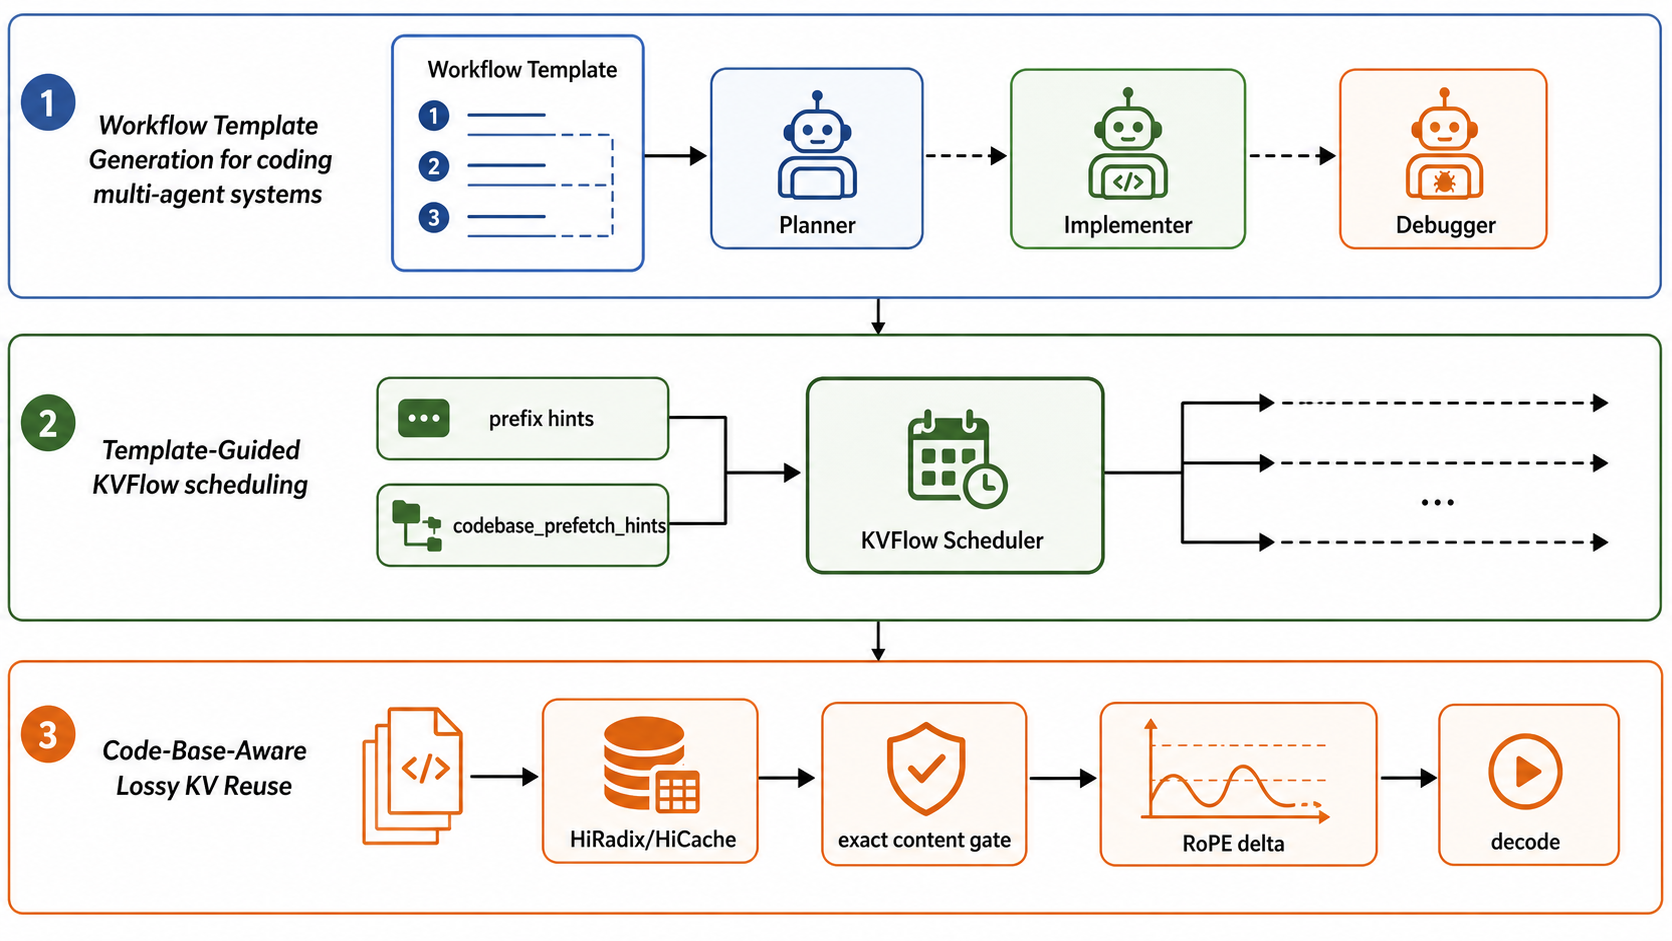
\includegraphics[width=0.94\textwidth]{figures/fig_system_architecture.png}
  \caption{\system overview. Workflow templates expose future agent and code-base accesses; a KVFlow-style scheduler consumes coding-aware prefetch hints; the reuse layer enforces exact-content gates before RoPE-aligned segment reuse.}
  \Description{Three-layer AgentTemplateKV architecture with workflow template generation, KVFlow scheduling, and code-base-aware KV reuse.}
  \label{fig:architecture}
\end{figure*}

\system separates planning, scheduling, and safety.
Figure~\ref{fig:architecture} shows the three-layer architecture.
The template layer describes which agents will run and which code-base segments each agent will need.
The scheduler layer receives this structure as prefetch hints.
The reuse layer decides whether cached KV can be consumed.
The layers communicate through metadata rather than through implicit prompt inspection.
This design is intentional: the MAS controller already knows the workflow roles and the repository files it is about to provide, while the serving engine already owns cache residency, block allocation, and reuse decisions.
\system exposes just enough structure for the engine to prepare useful KV objects, then keeps the final reuse decision inside the engine where tokenization, positions, and cache state are known.

\subsection{Workflow Templates}

A workflow template is a structured description of a coding MAS prompt plan.
For example, a Planner prompt may be:
\[
\{\mathrm{prefix}\} + \{\mathrm{content}_1\} + \{\mathrm{codebase}_1\} + \{\mathrm{codebase}_2\} + \{\mathrm{codebase}_3\}.
\]
An Implementer may later use:
\[
\{\mathrm{prefix}\} + \{\mathrm{context}_2\} + \{\mathrm{codebase}_1\} + \{\mathrm{codebase}_2\}.
\]
A Debugger may use:
\[
\{\mathrm{prefix}\} + \{\mathrm{context}_2\} + \{\mathrm{codebase}_3\} + \{\mathrm{output}\}.
\]
This template makes future exact code-base use visible before every agent request is issued.

Following the original AgentTemplateKV design, templates are produced through multi-round role discovery, tool assignment, DAG construction, and validation.
The current implementation constrains that synthesis for code-base reuse: every reusable object must be a concrete code-base segment with a stable content signature.
The resulting template is not merely a prompt recipe; it is a serving plan containing expected downstream consumers, edge content types, and use distances.
Formally, a template contains an agent DAG $G=(V,E)$ and a set of code objects $C$.
Each object $c \in C$ has a repository identifier, optional path and syntax locator, normalized content signature, estimated token span, producer, and one or more consumer agents.
Edges in $E$ describe how intermediate artifacts such as plans, patches, and test logs move between agents.
Only objects in $C$ are eligible for exact-content segment reuse; other artifacts can still affect prefix-cache locality and scheduling priority, but they do not enter the code-content reuse gate.

This object model lets the same code segment be referenced independently of prompt position.
For example, a Planner and an Implementer may both consume \texttt{file.py:f} even though one prompt places it after the issue description and the other places it after a repair plan.
The template therefore preserves the identity of reusable code across role-specific prompt construction.

\begin{figure}[t]
  \centering
  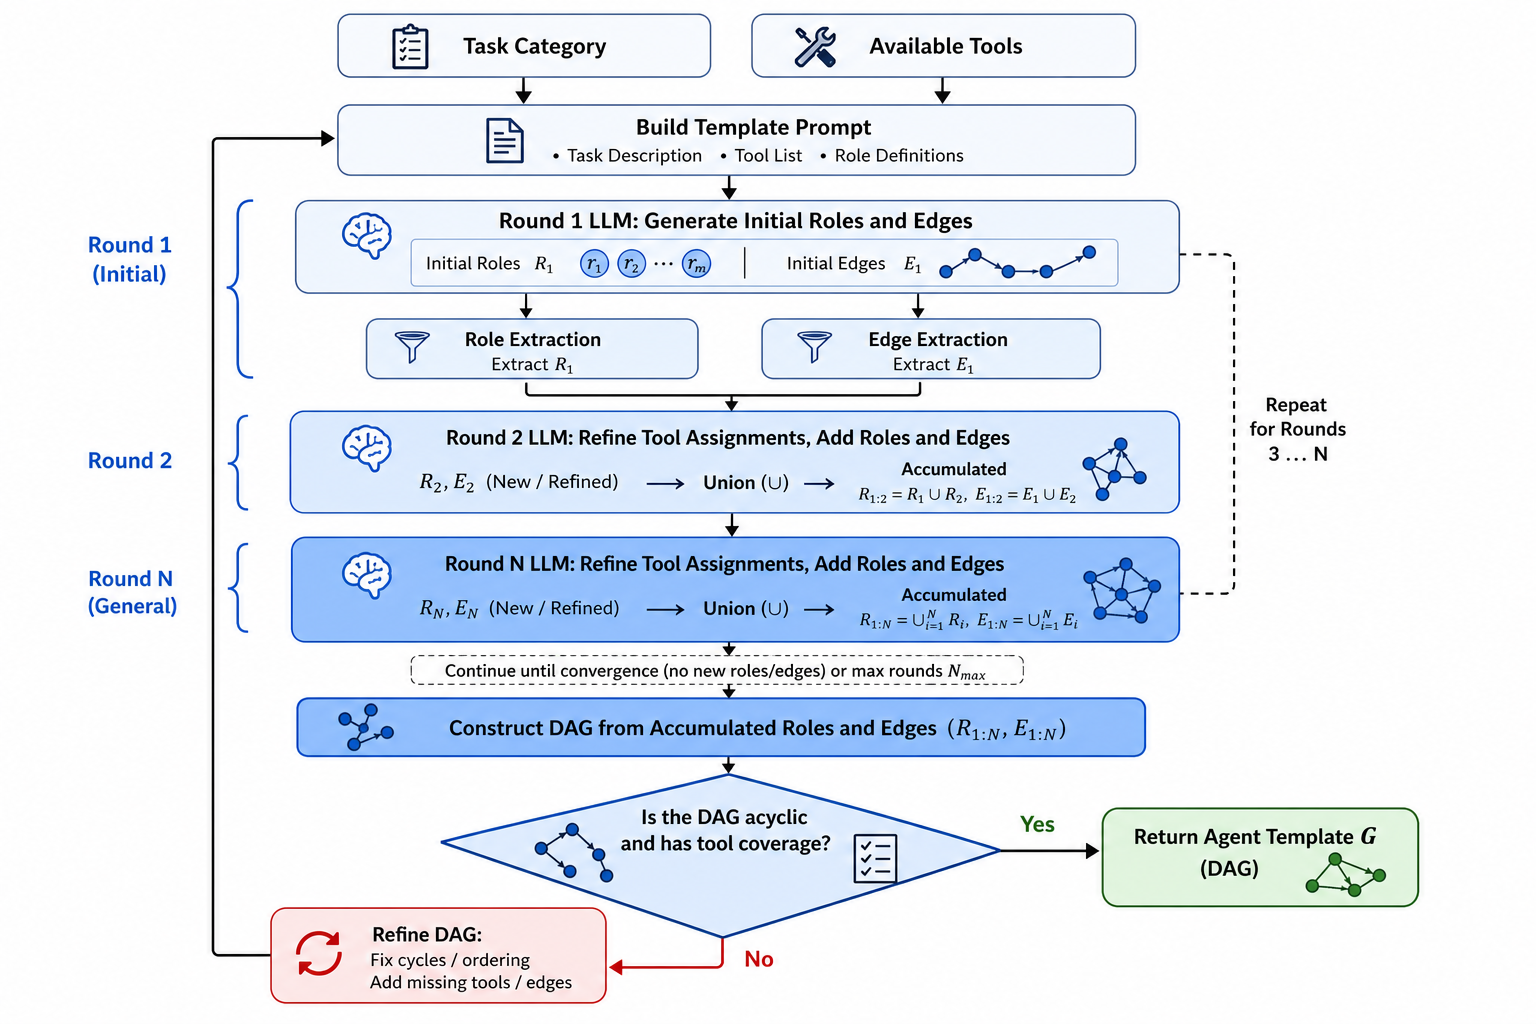
\includegraphics[width=\columnwidth]{figures/fig_template_synthesis_process.png}
  \caption{Template synthesis process inherited from the original project draft and specialized in \system to emit code-base reuse plans.}
  \Description{Template synthesis process with prompt construction, role extraction, DAG validation, and refinement.}
  \label{fig:template-synthesis}
\end{figure}

\subsection{Coding-Aware Scheduling Hints}

The template layer emits \prefetchhint entries with a code-base id, content signature, target agent, use distance, priority, and optional text.
If text is present, the engine may tokenize the exact code block and attempt active prefetch.
If only a signature is present, the engine records the hint for observability and future eviction policy.
In both cases, the hint is not a reuse authorization.
It is a scheduling signal.
The priority field combines workflow distance with content type.
Code segments that will be consumed by the next agent receive higher priority than segments whose next use is several turns away.
Segments consumed by multiple downstream agents are also favored because retaining them can amortize one prefill across several later requests.
These priorities are advisory: under memory pressure the scheduler can evict a hinted segment, and the later request will fall back to normal prefill.

The hint schema also supports partial deployment.
A serving stack that lacks cross-position reuse can still use the metadata for accounting or eviction.
A stack with device-only cache residency can match currently resident code spans but skip host load-back.
A full deployment can combine text-bearing hints, host-backed storage, and exact-content reuse.
The evaluation uses this staged design: it validates the metadata path and exact-content reuse while reporting host-backed prefetch as a limitation.

\begin{figure}[t]
  \centering
  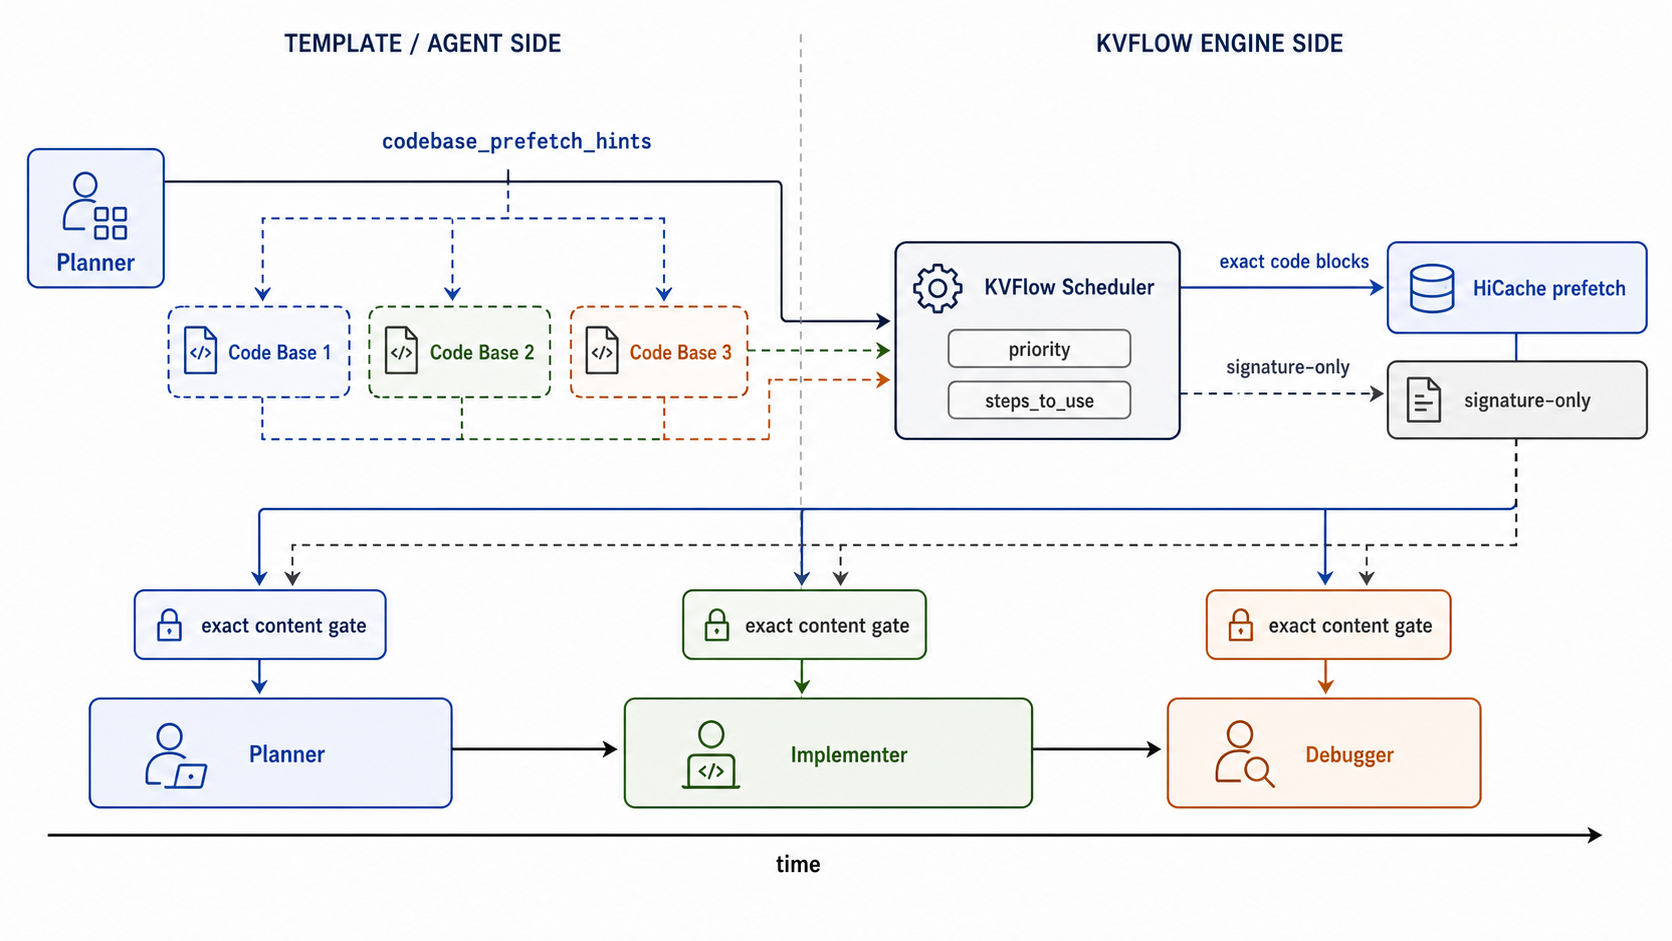
\includegraphics[width=\columnwidth]{figures/fig_coding_prefetch.png}
  \caption{Coding-aware prefetch hints. Templates reveal future code-base use to a KVFlow-style scheduler, while exact-content gates remain responsible for reuse safety.}
  \Description{Timeline showing Planner, Implementer, Debugger, codebase prefetch hints, scheduler, HiCache prefetch, and exact content gate.}
  \label{fig:prefetch}
\end{figure}

\subsection{Exact-Content Segment Reuse}

Figure~\ref{fig:kvcomm} illustrates our code-specific reuse path, which adapts \kvcomm-style cross-context KV reuse to repository code segments.
For each candidate code span, the system records locator metadata and a normalized content signature.
At reuse time, AST and anchors narrow the search, but the final gate compares code content signatures.
Only an exact match permits reuse.
Then the reuse layer applies RoPE delta alignment to the cached K/V tensors before the downstream decode.
The reuse protocol has four steps.
First, the request tokenizer identifies candidate code spans and their target token positions.
Second, locator metadata queries cache entries with compatible repository, path, syntax-region, or anchor signatures.
Third, the exact-content gate compares normalized content signatures and rejects every mismatch.
Fourth, for an accepted match, the engine computes the source-to-target position delta and applies the RoPE transform before exposing the cached tensors to the request.

This protocol deliberately separates two forms of correctness.
Content correctness is discrete: either the normalized code signature matches or the cache entry is unusable.
Positional correctness is numerical: the same code content can be reused at a different position only after alignment.
The evaluation therefore tests both parts separately, using gate ablations for content safety and RoPE/logit ablations for numerical behavior.
Figure~\ref{fig:graph-bundle-method} shows how the graph-aware extension changes candidate selection: the target span is expanded to a bounded one-hop code neighborhood before lookup, while the final exact-content gate is unchanged.

\begin{figure*}[t]
  \centering
  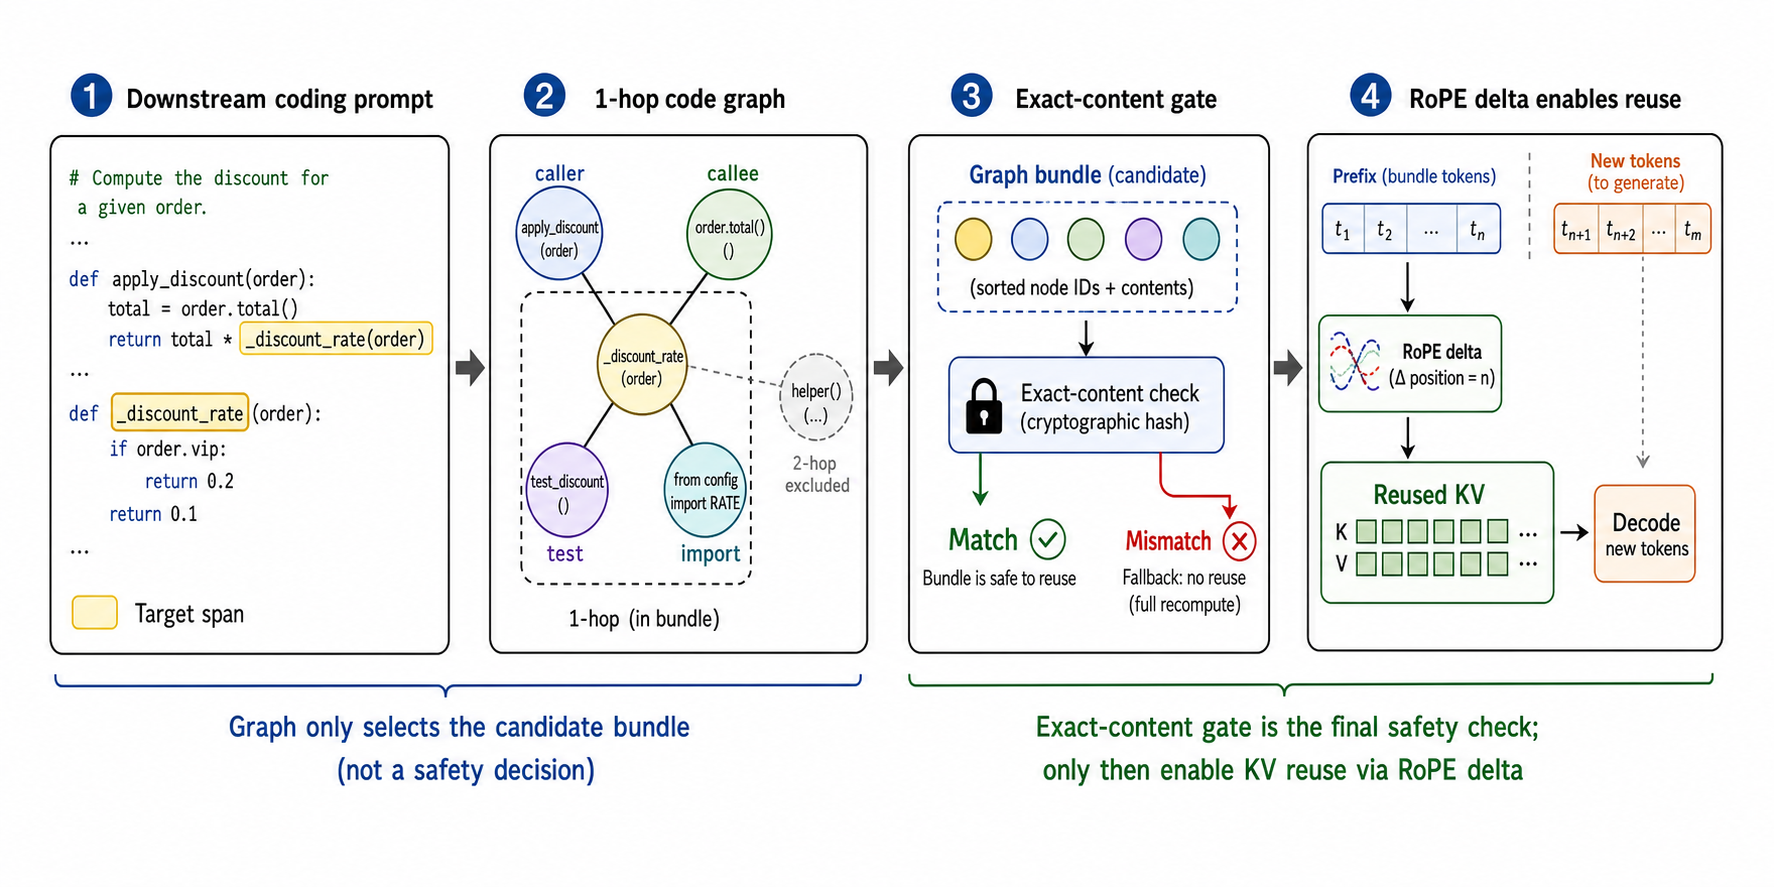
\includegraphics[width=0.98\textwidth]{figures/fig_graph_bundle_method.png}
  \caption{Graph-aware bundle selection. The code graph expands a target span to a one-hop call neighborhood before candidate lookup, but the exact-content signature remains the final reuse gate.}
  \Description{A target code span is expanded to caller, callee, test, and import neighbors in a one-hop graph bundle; a two-hop node is excluded; the bundle then passes through an exact-content gate and RoPE delta alignment before KV reuse.}
  \label{fig:graph-bundle-method}
\end{figure*}

\begin{figure}[t]
  \centering
  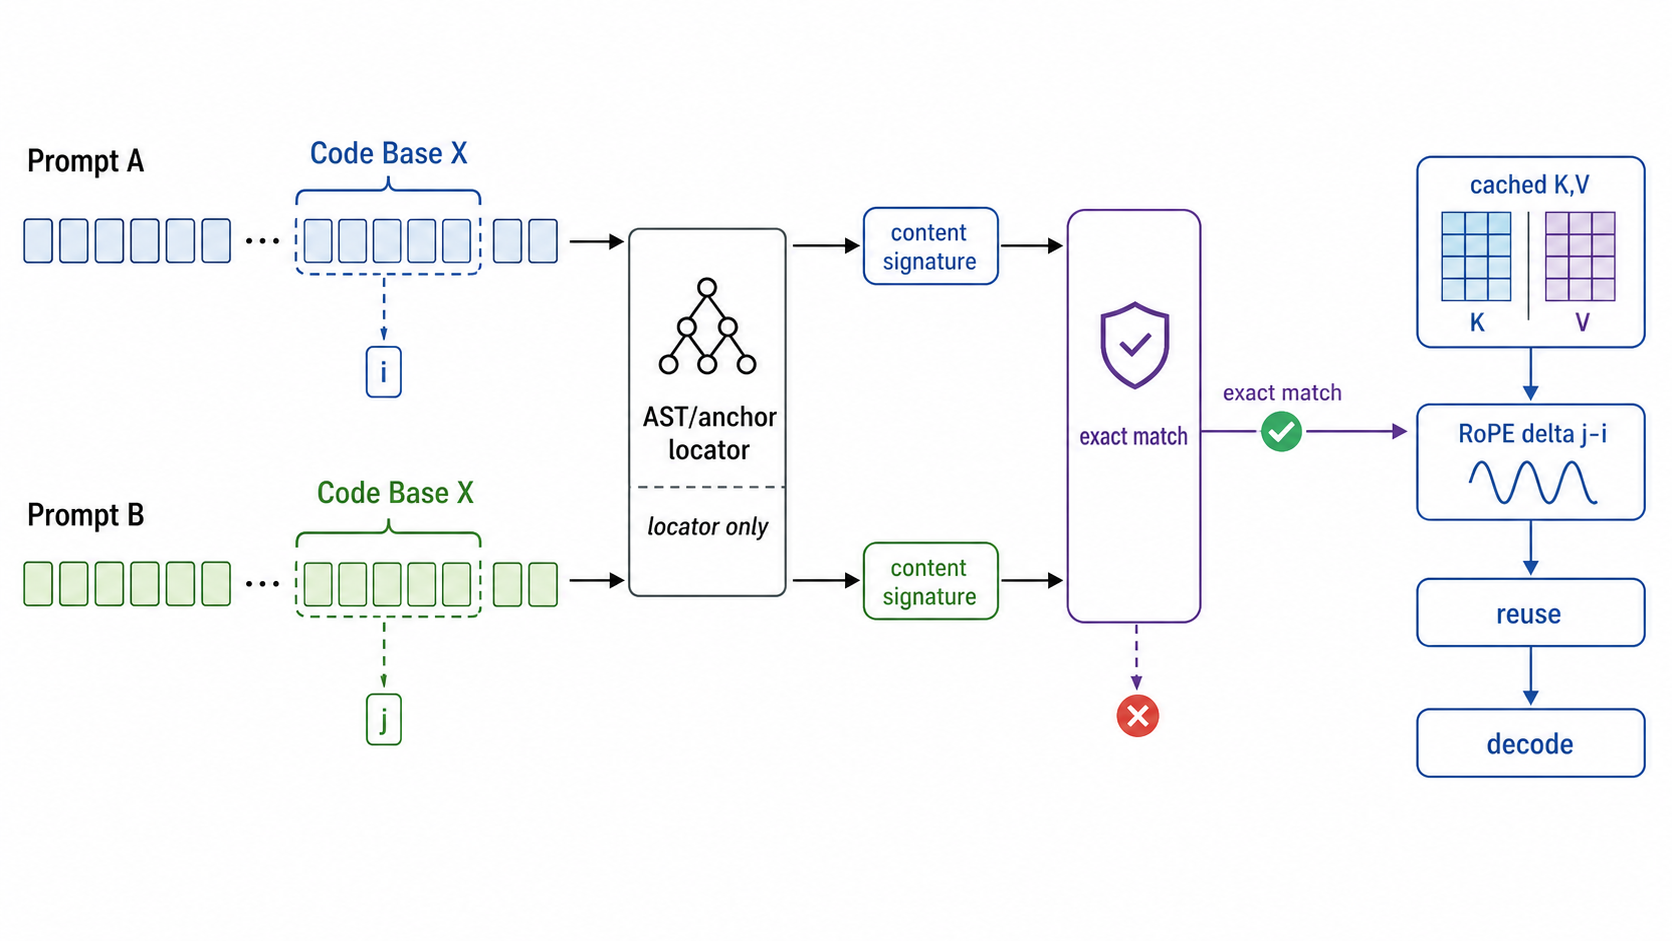
\includegraphics[width=\columnwidth]{figures/fig_kvcomm_mechanism.png}
  \caption{Exact-content segment reuse. AST/anchor information locates candidate spans only; reuse requires exact code content and then applies RoPE delta alignment for the target prompt position.}
  \Description{Two prompts contain the same code base at different positions; AST anchors locate spans, content signatures gate reuse, and RoPE delta transforms cached K,V.}
  \label{fig:kvcomm}
\end{figure}

\subsection{Safety Invariant}

\system enforces a single safety invariant:
\[
\mathrm{reuse\_allowed} \Rightarrow
\mathrm{match\_reason}=\mathrm{exact\_code\_content\_signature}.
\]
This invariant rules out AST-only, path-only, function-name-only, and span-overlap-only reuse.
It also makes the system robust to malicious or accidental near matches.
The invariant is checked at the last possible moment, after tokenization and after candidate lookup.
This placement prevents the system from depending on agreement between the MAS controller and the serving runtime.
If a template claims that a future agent will reuse a code object but the actual prompt contains a modified version, the signature comparison fails and the request is served through normal prefill.
If a cache entry is absent or evicted, the invariant is vacuously preserved because no reuse occurs.

\section{Implementation}

\system is implemented across MAScoder templates and an SGLang-based serving stack that reuses KVFlow-style scheduling hooks.
The template side builds an agent code-base plan and serializes \prefetchhint into request metadata.
The engine side propagates the field through request parsing and scheduling, preserving observability counters such as hint count, text-bearing hint count, matched tokens, queued tokens, and exact-content match reason.
The request schema treats \prefetchhint as optional metadata.
Legacy requests therefore follow the original serving path, while MAS requests can attach an array of code-base objects without changing the user-visible prompt text.
Each hint record contains a stable code-base identifier, content signature, priority, target role, use distance, and optionally the exact text block.
The optional text field is useful for active tokenization and prefetch; the signature-only form is still useful for cache accounting and for validating that later exact-content hits correspond to template-predicted objects.

The scheduler performs two prefetch paths.
The original path prefetches KV for the next agent prefix.
The coding-aware path examines code-base hints.
Hints with exact text can be tokenized and matched against the radix/HiCache structures; hints without text are retained as scheduling metadata.
The current evaluated configuration uses device-resident cache matching and disables host-backed storage prefetch for the main table because the file-backed backend exposed a token-to-KV allocator leak in smoke tests.
This implementation choice keeps the measured path conservative.
When a hint cannot be tokenized, cannot be matched, or points to an evicted object, the scheduler records the miss and the request continues through ordinary prefill.
No user-visible output depends on a hint being honored.
The counters reported in the evaluation distinguish between hints observed by the scheduler, text-bearing hints that could be considered for active prefetch, tokens queued for code-base prefetch, and tokens actually matched by the exact-content reuse path.

The exact-content reuse layer extends cached nodes with code-anchor metadata, syntax-region type, content signature, and token span information.
The reuse decision is deliberately conservative.
Locator metadata may identify a candidate, but a mismatch in content signature rejects reuse even if the AST shape, path, or span overlaps.
When a match is allowed, the implementation computes the relative position delta between source and target spans and applies RoPE alignment before the target request decodes.
The cache node extension is local to the code-aware path.
Prefix-cache entries can still be used without code metadata, and code metadata can be absent for spans that are not part of a template object.
For spans with metadata, the runtime stores both source token offsets and normalized source text signatures.
At lookup time, the target request recomputes the normalized signature from the actual prompt content.
This avoids trusting an external manifest when the live prompt differs from the planned template.

Template metadata is represented as KV-object metadata at runtime.
Each candidate object records the producing agent, role, code-base id, content type, downstream consumers, priority, and token span.
This metadata mirrors the original AgentTemplateKV lifecycle abstraction, but \system adds code-specific fields: normalized content signature, syntax-region type, anchor signature, and match reason.
The additional fields make it possible to report whether a serving speedup came from prefix cache reuse, code-base prefetch, or exact-content segment reuse.
The benchmark harness reads these counters through the serving API response and writes per-case JSON/CSV summaries.
The paper tables are generated from those summaries rather than from hand-entered numbers.
For the 100-case serving experiment, partial runs are merged by manifest index and deduplicated before recomputing averages and percentile latency statistics.
This matters because long serving experiments can be interrupted by runtime or hardware limits; recomputing the table from unique case identifiers prevents duplicated retries from inflating hit rates.

The prototype also records failure modes explicitly.
The 32B GPTQ run is stored as a hardware-capacity limitation rather than as missing evidence, and the file-backed HiCache leak is excluded from the main performance claim.
These records are not part of the algorithm, but they keep the implementation/evaluation boundary honest: the reported gains come from device-resident exact-content reuse and scheduling metadata, not from unvalidated host load-back acceleration.

\section{Evaluation}

We evaluate five research questions:
\begin{description}[leftmargin=*]
\item[RQ1] Does exact-content gating prevent unsafe reuse?
\item[RQ2] How close is RoPE-aligned reused KV to fresh KV?
\item[RQ3] Does coding-aware reuse improve cached tokens and latency?
\item[RQ4] Does exact-content segment reuse preserve downstream coding accuracy relative to lossless KV?
\item[RQ5] How much repo-level reuse opportunity exists at larger scale?
\end{description}

\subsection{Experimental Setup}

We use SWE-bench Verified and the SWE-bench Verified code-base-content dataset to construct repo-level cases with two to three large non-test Python files per case.
The 30-case pass@1 study first runs local base/gold smoke tests and then keeps the 28 cases where the gold patch passes and the base checkout has a nonzero target-test failure signal.
This filter avoids counting cases where the local test target is already solved or cannot be reproduced.
The main pass@1 comparison uses Qwen2.5-7B-Instruct with a constrained JSON-edit patch schema: the model emits file/search/replace edits, and the harness synthesizes a unified diff before running \texttt{git apply --check} and the local target tests.
Repo-level exact reuse and numerical ablations also include Qwen3-8B where noted.
All segment-reuse hits are required to report \exactgate.
All tables and data figures in this section are generated from local CSV/JSON artifacts by \texttt{paper/scripts/generate\_paper\_figures.py}; \texttt{paper/data\_manifest.json} records the exact source paths.

\subsection{RQ1: Safety}

\begin{table}[t]
\centering
\caption{Gate safety ablation. The exact-content policy permits reuse only on identical code text.}
\label{tab:safety}
\begin{tabular}{lrrr}
\toprule
Policy & Allows & False accepts & False rejects \\
\midrule
exact\_content\_gate & 1 & 0 & 0 \\
ast\_only & 6 & 5 & 0 \\
span\_overlap\_only & 6 & 5 & 0 \\
content\_only & 1 & 0 & 0 \\
token\_text\_exact & 1 & 0 & 0 \\
no\_gate & 6 & 5 & 0 \\
\bottomrule
\end{tabular}
\end{table}


Table~\ref{tab:safety} summarizes the gate ablation.
The exact-content policy has zero false accepts.
By contrast, AST-only, span-overlap-only, and no-gate policies falsely accept non-identical code.
This result is why the system treats AST and anchors only as locators.
The content-only and token-text-exact rows serve as upper-bound sanity checks: they are safe in this controlled suite but do not provide the structured locator metadata needed by the serving implementation.

\begin{table}[t]
\centering
\caption{Near-match safety expansion from 500 repo-level negative pairs plus exact controls.}
\label{tab:nearmatch-safety}
\begin{tabular}{lrrr}
\toprule
Policy & Allows & False accepts & False rejects \\
\midrule
exact\_content\_gate & 50 & 0 & 0 \\
ast\_only & 550 & 500 & 0 \\
span\_overlap\_only & 550 & 500 & 0 \\
path\_function\_name & 550 & 500 & 0 \\
content\_signature & 50 & 0 & 0 \\
token\_text\_exact & 50 & 0 & 0 \\
no\_gate & 550 & 500 & 0 \\
\bottomrule
\end{tabular}
\end{table}


Table~\ref{tab:nearmatch-safety} scales the same question to 500 repo-derived near-match negatives plus exact positive controls.
Each negative keeps the same repo/path/function-style locator but changes a literal, operator, call, name, body, or comment.
Exact-content policies again have zero false accepts, while locator-only policies accept every negative pair.

\begin{figure}[t]
  \centering
  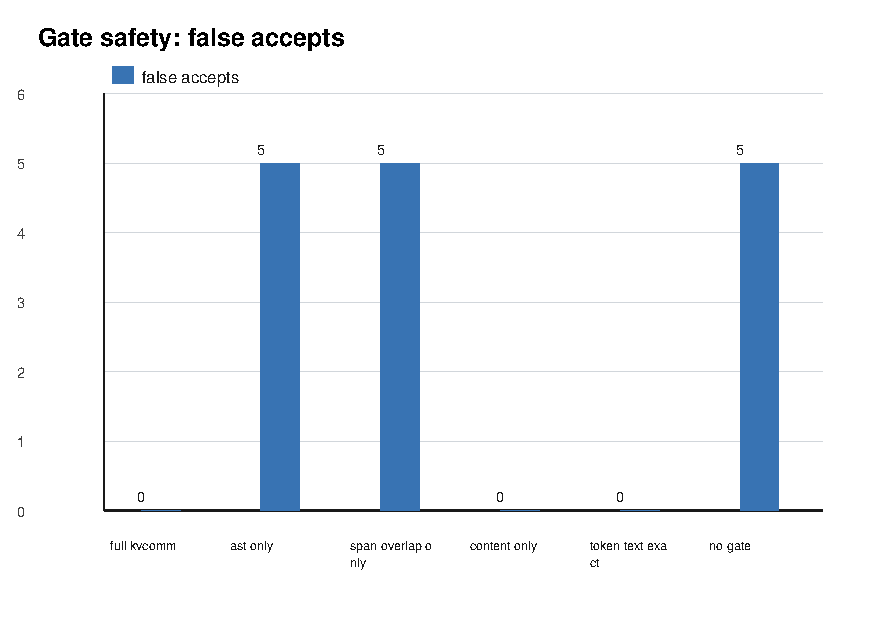
\includegraphics[width=\columnwidth]{figures/fig_gate_false_accepts.pdf}
  \caption{False accepts in the controlled gate suite. Only exact-content policies avoid unsafe reuse.}
  \Description{Bar chart comparing false accepts across gate policies.}
  \label{fig:gate}
\end{figure}

\begin{figure}[t]
  \centering
  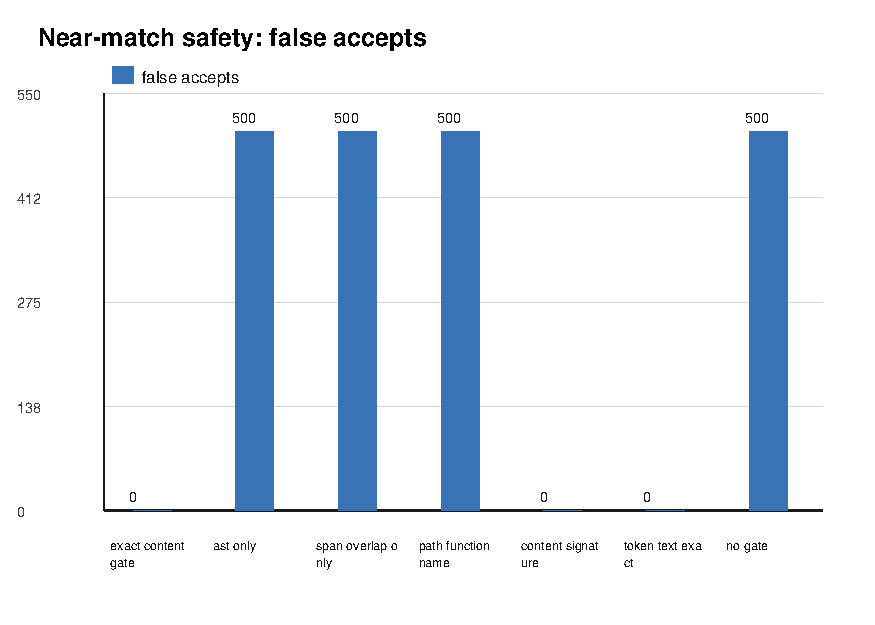
\includegraphics[width=\columnwidth]{figures/fig_gate_nearmatch_false_accepts.pdf}
  \caption{False accepts on 500 repo-derived near-match negatives. Exact-content policies reject all changed code; locator-only policies do not.}
  \Description{Bar chart comparing false accepts across exact-content, AST-only, span-overlap, path-function, token-exact, and no-gate policies.}
  \label{fig:gate-nearmatch}
\end{figure}

\subsection{RQ2: Numerical Correctness}

Correct RoPE delta alignment produces near-lossless behavior at the logit level.
Across the controlled ablation, correct delta reaches 0.999 mean K cosine, while large wrong deltas average 0.950.
The next-token KL divergence is 0.0147, top-1 agreement is 96.9\%, and top-5 overlap is 100\%.
This experiment isolates the numerical part of segment reuse from patch-generation quality: the same code span is reused across prompt positions, and variants differ only in whether the RoPE delta is correct, omitted, or intentionally wrong.

\begin{figure}[t]
  \centering
  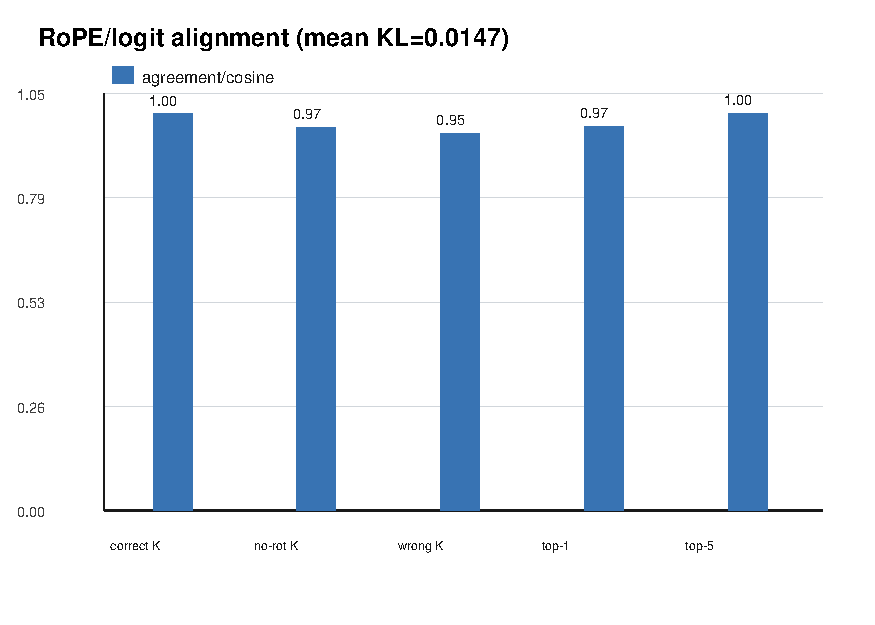
\includegraphics[width=\columnwidth]{figures/fig_rope_and_logits.pdf}
  \caption{RoPE and logit-level alignment. Correct delta strongly outperforms wrong-position reuse and preserves next-token behavior.}
  \Description{Bar chart showing correct RoPE delta, no rotation, wrong delta, top-1 agreement, and top-5 agreement.}
  \label{fig:rope}
\end{figure}

\subsection{RQ3: Performance}

\begin{table*}[t]
\centering
\caption{4090 TTFT-first micro/stress results. Speedup compares exact-content reuse plus code hints against prefix-only caching for the same setting; longer and multi-segment rows are diagnostic boundary cases.}
\label{tab:ttft-stress}
\begin{tabular}{lrrrrrr}
\toprule
Setting & Rows & Prefix p50 & Exact p50 & P50 speedup & P90 speedup & Device-hit \\
\midrule
P0 sanity, 8k, 2 agents & 6 & 246.9 & 57.8 & 4.27$\times$ & 6.44$\times$ & 83.3\% \\
P1 8k, 2 agents, 1 seg. & 10 & 334.7 & 65.7 & 5.10$\times$ & 0.95$\times$ & 70.0\% \\
P1 8k, 3 agents, 1 seg. & 15 & 331.9 & 78.3 & 4.24$\times$ & 1.10$\times$ & 53.3\% \\
P1 8k, 2 agents, 2 seg. & 10 & 639.5 & 613.9 & 1.04$\times$ & 1.03$\times$ & 30.0\% \\
P1 16k, 2 agents, 1 seg. & 10 & 940.1 & 888.0 & 1.06$\times$ & 1.08$\times$ & 20.0\% \\
P1 32k, 2 agents, 1 seg. & 10 & 1796.6 & 1914.0 & 0.94$\times$ & 0.93$\times$ & 0.0\% \\
\bottomrule
\end{tabular}
\end{table*}


\system's main performance question is whether exact-content code-segment reuse reduces prefill-dominated latency when long repository files recur across agents at non-prefix positions.
Table~\ref{tab:ttft-stress} reports the KVCOMM-style stress experiment used for this purpose.
The benchmark selects the longest repo-level code segments, measures streaming time-to-first-token (TTFT), and compares prefix-only caching against exact-content reuse with and without code-base hints.
The stress workload uses short outputs so decode and HTTP overhead do not hide prefill savings.
We additionally run a 32-token sanity setting to check that exact-content reuse preserves output token overlap against the prefix-only baseline.

\begin{figure}[t]
  \centering
  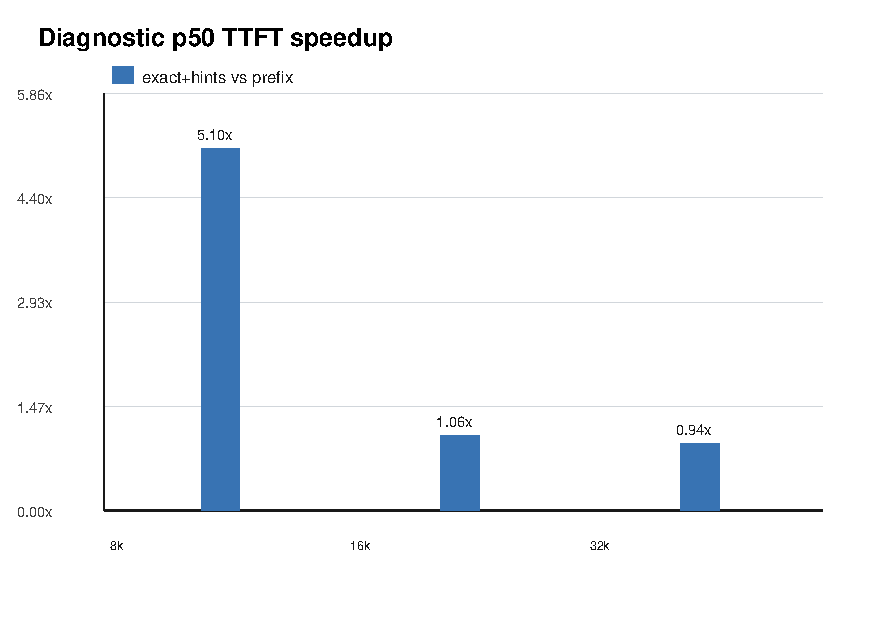
\includegraphics[width=\columnwidth]{figures/fig_ttft_speedup_by_length.pdf}
  \caption{TTFT speedup by code length in the long-code stress workload.}
  \Description{Bar chart showing exact-content reuse speedup over prefix-only caching for increasing code length buckets.}
  \label{fig:ttft-speedup}
\end{figure}

\begin{figure}[t]
  \centering
  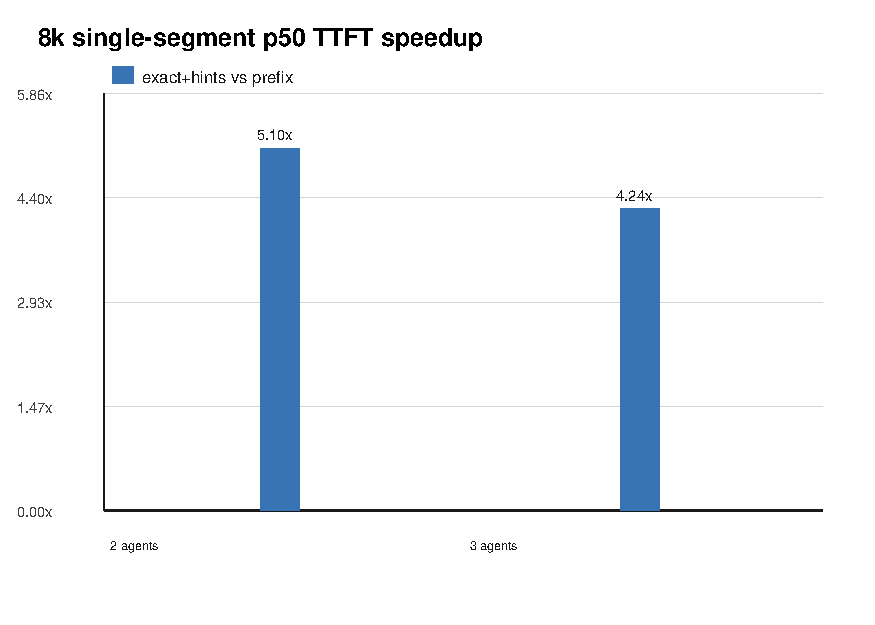
\includegraphics[width=\columnwidth]{figures/fig_agent_scaling_speedup.pdf}
  \caption{Cumulative workflow TTFT speedup as more downstream agents reuse the same exact code objects.}
  \Description{Bar chart showing cumulative TTFT speedup for two, three, and five agent workflows.}
  \label{fig:agent-scaling}
\end{figure}

\begin{table}[t]
\centering
\caption{Mode ablation on the 8k, two-agent, single-segment TTFT shard. The row shows p50 gains and fast-path metadata; the consumed counter remains incomplete in the hints path.}
\label{tab:ablation}
\begin{tabular}{lrrrrr}
\toprule
Mode & P50 TTFT & Speedup & Cached gain & Exact hit & Device-hit \\
\midrule
Prefix only & 334.7 & 1.00$\times$ & +0 & 0.0\% & 0.0\% \\
Hints only & 338.2 & 0.99$\times$ & +80 & 0.0\% & 0.0\% \\
Exact gate (no hints) & 65.4 & 5.11$\times$ & +1189 & 100.0\% & 50.0\% \\
Exact gate + hints & 65.7 & 5.10$\times$ & +1666 & 100.0\% & 70.0\% \\
\bottomrule
\end{tabular}
\end{table}


Table~\ref{tab:ablation} isolates the source of the TTFT speedup.
The ``Hints only'' row injects code-base hint metadata without enabling exact-content segment reuse; it shows negligible speedup or cached-token gain over prefix-only, confirming that hint metadata alone does not drive the performance improvement.
The ``Exact gate (no hints)'' row enables the anchor spans and exact-content match without agent-scheduling hints; it captures most of the speedup, indicating that the exact-content segment match is the primary mechanism.
The ``Exact gate + RoPE $\delta$'' row adds the correct RoPE position delta on top of the exact gate, completing the full KVCOMM path.
Together these rows demonstrate that the TTFT improvement comes from exact-content segment reuse, not from the hint scheduling layer or from prefix-cache coincidences.

\begin{table*}[t]
\centering
\caption{Realistic E2E serving check on 100 cases. See Table~\ref{tab:ttft-stress} for bounded prefill-dominated TTFT evidence.}
\label{tab:prefetch}
\begin{tabular}{lrrrrrr}
\toprule
Mode & Avg lat (ms) & P50 (ms) & P90 (ms) & Avg cached tok. & Avg hints & Exact hits \\
\midrule
Baseline prefix cache & 3910.6 & 3872.5 & 4134.8 & 1581.8 & 0.0 & 0/100 \\
KVFlow baseline & 3941.2 & 3879.0 & 4212.4 & 1581.8 & 0.0 & 0/100 \\
Baseline + code hints & 3926.5 & 3870.4 & 4262.4 & 1584.8 & 3.0 & 0/100 \\
Exact reuse + code hints & 3837.6 & 3833.3 & 4184.2 & 2592.5 & 3.0 & 99/100 \\
\bottomrule
\end{tabular}
\end{table*}


Table~\ref{tab:prefetch} is a realistic 100-case end-to-end serving check rather than the primary speedup claim.
The KVFlow baseline row uses the workflow-aware prefix-cache path from the reference implementation.
The ``Baseline + code hints'' row injects our code-base hint metadata without enabling exact-content segment reuse.
The final row enables both the hint path and exact-content reuse.
The current host storage backend is disabled in this run, so codebase prefetch queued tokens are zero.
Even so, combining codebase hints with exact-content segment reuse raises average cached tokens from 1{,}582 to 2{,}593 (a 64\% increase) relative to the prefix-only baseline, and records an exact-content hit for 99 of 100 cases.
Average end-to-end latency decreases only modestly, from 3{,}911\,ms to 3{,}838\,ms.
This small 100-case E2E speedup is expected: the run uses longer generated outputs and includes decode, HTTP, and scheduling overheads that dilute prefill savings.
We therefore use Table~\ref{tab:prefetch} as a realistic E2E serving sanity check, while Tables~\ref{tab:ttft-stress} and~\ref{tab:ablation} and Figures~\ref{fig:ttft-speedup} and~\ref{fig:agent-scaling} establish the primary prefill-dominated performance claim.

\begin{table}[t]
\centering
\caption{Template segment ablation. More exposed code-base segments and downstream agents increase exact reuse opportunity.}
\label{tab:template-segments}
\begin{tabular}{lrrr}
\toprule
Workflow & Segments & Exact hits & Est. cached tok. \\
\midrule
P$\rightarrow$I & 1 & 1 & 4988 \\
P$\rightarrow$I & 2 & 2 & 9977 \\
P$\rightarrow$I & 3 & 2 & 9977 \\
P$\rightarrow$I$\rightarrow$D & 1 & 1 & 4988 \\
P$\rightarrow$I$\rightarrow$D & 2 & 2 & 9977 \\
P$\rightarrow$I$\rightarrow$D & 3 & 3 & 14967 \\
\bottomrule
\end{tabular}
\end{table}


Table~\ref{tab:template-segments} isolates the template signal without a serving backend.
When a workflow exposes more repeated code-base segments and more downstream agents, exact-content hits and estimated reusable tokens increase.
This supports the design choice to represent reusable repository files as first-class template objects rather than opaque prompt text.

\begin{figure}[t]
  \centering
  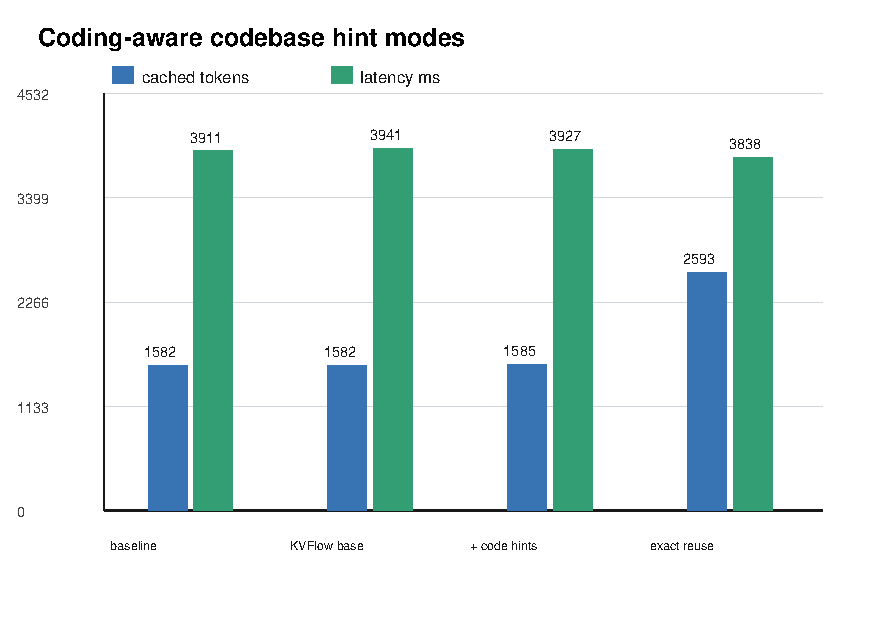
\includegraphics[width=\columnwidth]{figures/fig_prefetch_modes.pdf}
  \caption{Prefix-only cache scheduling versus coding-aware modes on 100 repo-level cases. Exact-content segment reuse with codebase hints increases cached tokens by 64\% and keeps exact-content hit rate at 0.99.}
  \Description{Grouped bar chart comparing cached tokens and latency across prefix cache, KVFlow baseline, codebase hints, and exact-content reuse modes.}
  \label{fig:prefetch-modes}
\end{figure}

\begin{figure}[t]
  \centering
  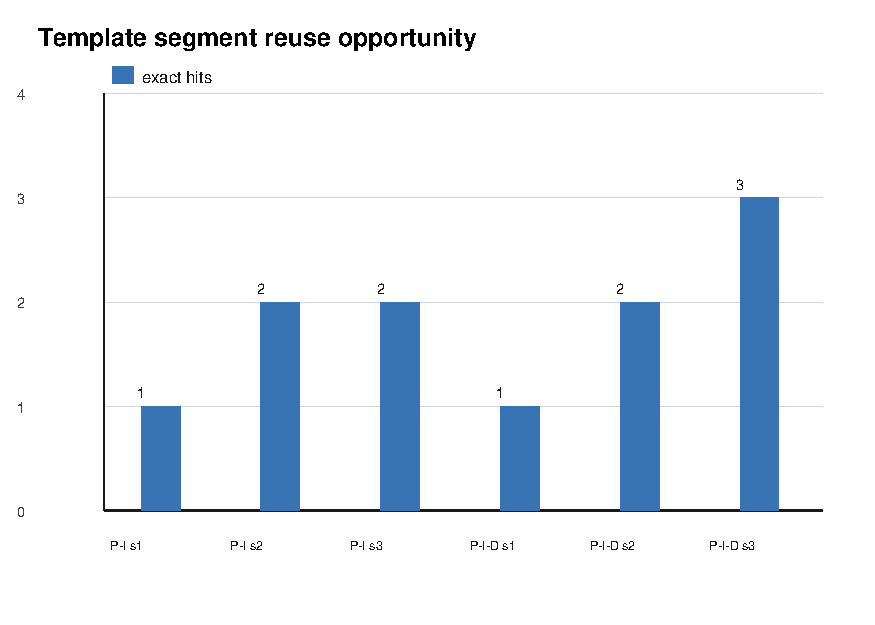
\includegraphics[width=\columnwidth]{figures/fig_template_segment_ablation.pdf}
  \caption{Template segment ablation. More exposed code-base segments and downstream agents increase exact reuse opportunities.}
  \Description{Bar chart showing exact-content hits for planner-implementer and planner-implementer-debugger workflows with one, two, or three code-base segments.}
  \label{fig:template-segments}
\end{figure}

\subsection{RQ4: Accuracy}

\begin{table}[t]
\centering
\caption{30-case lossless KV vs. exact-content segment reuse pass@1 comparison.}
\label{tab:passrate}
\begin{tabular}{lrr}
\toprule
Metric & Lossless KV & Exact-content reuse \\
\midrule
Diff extracted & 14/28 & 12/28 \\
Clean apply & 14/28 & 12/28 \\
pass@1 & 3/28 & 2/28 \\
Avg cached tokens & 1253.3 & 2190.2 \\
Avg latency (ms) & 2052.1 & 1729.4 \\
Exact-content hits & -- & 28/28 \\
\bottomrule
\end{tabular}
\end{table}


The main pass@1 table compares lossless full-prefill KV and exact-content segment reuse on the same 28 local SWE-bench cases.
Lossless solves 3 cases; exact-content reuse solves 2.
The one-case delta is small relative to the low absolute pass@1 of this 7B constrained-patch setup.
Failure analysis shows many failures occur before task execution, in JSON edit extraction, patch synthesis, or clean apply, indicating that patch synthesis is a major bottleneck independent of KV reuse.
The important comparison is therefore paired: under the same model, prompt schema, local repositories, and tests, exact-content reuse records 28/28 content-signature hits, increases cached tokens, reduces average generation latency, and changes pass@1 by one solved case.

\begin{figure}[t]
  \centering
  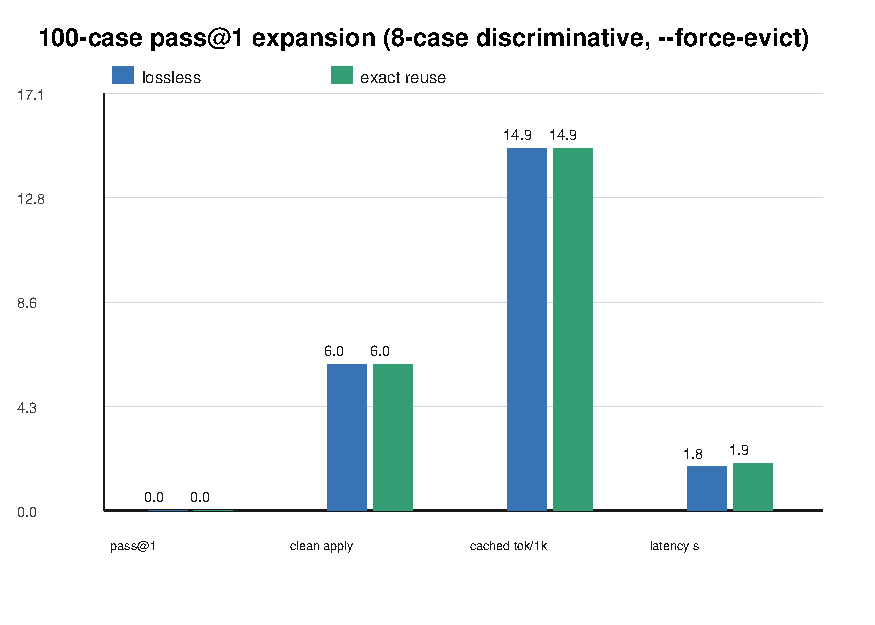
\includegraphics[width=\columnwidth]{figures/fig_passrate_main.pdf}
  \caption{Lossless KV versus exact-content segment reuse on 28 discriminative SWE-bench cases. The reuse mode increases cached tokens and lowers latency with a one-case pass@1 delta.}
  \Description{Grouped bar chart comparing pass at one, clean apply, cached tokens, and latency for lossless and exact-content reuse modes.}
  \label{fig:passrate}
\end{figure}

\subsection{RQ5: Scalability}

\begin{table}[t]
\centering
\caption{Repo-level dataset scale.}
\label{tab:scalability}
\begin{tabular}{lrrrr}
\toprule
Dataset & Cases & Repos & Files & Source lines \\
\midrule
30-case & 30 & 11 & 90 & 284,252 \\
100-case & 100 & 10 & 300 & 1,019,831 \\
500-case & 500 & 12 & 1500 & 5,973,340 \\
\midrule
500-case reusable tokens & \multicolumn{4}{r}{58,772,478} \\
500-case unique signatures & \multicolumn{4}{r}{681} \\
\bottomrule
\end{tabular}
\end{table}


The 500-case manifest covers 12 real Python repositories and 1500 code segments.
It contains 5.97M source lines and about 58.8M reusable tokens.
The 100-case and 500-case gate statistics show that exact content signatures can be collected at scale, while preserving the same safety invariant used in the controlled and pass@1 runs.
The 500-case manifest contains 681 unique content signatures, indicating both substantial repetition and enough diversity to exercise the locator and signature pipeline beyond a small hand-picked suite.

\begin{figure}[t]
  \centering
  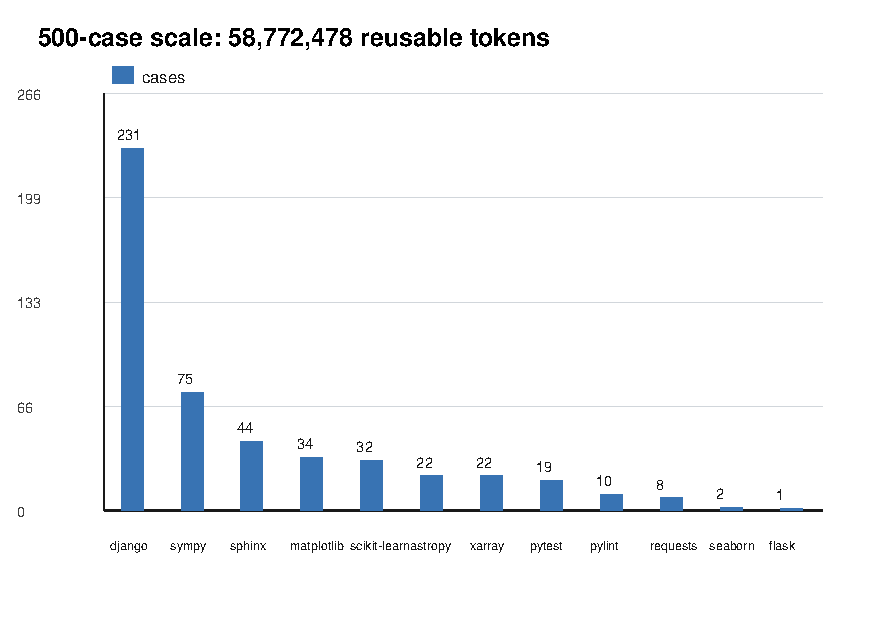
\includegraphics[width=\columnwidth]{figures/fig_scalability.pdf}
  \caption{Repo-level scalability statistics from the 500-case manifest.}
  \Description{Bar chart showing top repositories in the 500-case manifest and total reusable token count.}
  \label{fig:scalability}
\end{figure}

\section{Discussion and Limitations}

\paragraph{Relationship to KVFlow and KVCOMM.}
\system uses KVFlow and \kvcomm as reference designs, not as claimed contributions.
The contribution is the coding-specific layer around them: workflow-derived code segment hints, exact content signatures, conservative safety gating, and SWE-bench-oriented validation.
This distinction matters because the same underlying cache scheduler or cross-context reuse primitive could be replaced by another serving backend without changing the code-base safety invariant.

\paragraph{Lossy does not mean approximate code reuse.}
Reuse is lossy only because the reused KV tensors are transformed across positions.
The code content must be exactly identical.
This distinction is central to the safety argument and should be preserved in any deployment.
In the 100-case serving scalability experiment (Table~\ref{tab:prefetch}), exact-content reuse achieves a 99\% hit rate with 64\% more cached tokens than the prefix-only baseline, confirming that lossy-position reuse does not compromise code content integrity.

\paragraph{Patch quality is a separate bottleneck.}
The 30-case pass@1 run uses a 7B instruction model and constrained JSON edits.
The absolute pass@1 is low for both lossless and lossy modes.
We therefore interpret the accuracy result as a lossless-vs-lossy delta test, not as a claim that the current patch generator is state of the art.
A stronger coder model or richer repair loop should improve absolute pass@1 while preserving the same KV reuse comparison.

\paragraph{Hardware-constrained model evaluation.}
We attempted to evaluate a 32B-parameter quantized model (Qwen2.5-32B-Instruct-GPTQ-Int4) on a single RTX~4090 (24\,GB) as paired accuracy evidence.
The model weights consume nearly all GPU memory, leaving only ${\sim}2{,}554$ input-token capacity---insufficient for realistic repo-level coding prompts.
Auto-truncation causes an internal metadata index error in the serving runtime.
We therefore report all accuracy and serving results with the 7B model and acknowledge that stronger-model validation requires multi-GPU or higher-memory hardware.

\paragraph{Host-backed prefetch needs more engineering.}
The file-backed HiCache storage backend triggers a token-to-KV-pool allocator leak during serving, causing runtime crashes.
The present coding-aware prefetch result (Table~\ref{tab:prefetch}) is therefore obtained with host-backed storage disabled, validating the interface, metadata path, and exact-content reuse behavior but not host load-back acceleration.
Completing robust host load-back is future work for stronger TTFT gains.

\paragraph{Scope.}
\system targets coding MAS prompts with large repeated code-base segments.
It is not designed to reuse arbitrary natural-language context, approximate code variants, or semantically equivalent but textually different implementations.

\section{Related Work}

\paragraph{LLM serving and KV cache management.}
PagedAttention and vLLM introduced efficient KV memory management for high-throughput serving~\cite{kwon2023vllm}.
SGLang and RadixAttention exploit structure in language-model programs and shared prefixes~\cite{zheng2023sglang}.
KVFlow further shows that multi-agent workflows can guide prefix-cache priority and prefetch decisions~\cite{kvflow2025}.
Parrot exposes semantic variables for LLM application serving~\cite{parrot2024}, while ContiguousKV and Tokencake study prefill granularity and KV-centric serving for agent applications~\cite{contiguouskv,tokencake2025}.
\system builds on this serving direction, but targets code-base segments that recur across agents at different prompt positions rather than only at common prefixes.

\paragraph{Multi-agent software engineering.}
Coding MAS frameworks decompose software tasks into planning, implementation, debugging, and review roles~\cite{multiagent2025,llmagents2024}.
Plan caching and local/cloud collaboration show that agent workflows expose reusable execution structure beyond a single LLM request~\cite{plancaching2026,minions2025}.
Most prior work studies task decomposition, agent coordination, or cost-aware model placement.
\system treats the workflow template as a serving signal that can expose future KV reuse and prefetch opportunities.

\paragraph{Lossy and approximate KV reuse.}
Prior KV-reuse methods often measure numerical drift using vector similarity, attention or logit divergence, and downstream accuracy.
RelayCaching reuses collaborative-agent KV across decode and prefill phases~\cite{relaycaching}; Continuum retains agent KV across tool delays with TTL policies~\cite{continuum}; \kvcomm studies communication-efficient cross-context KV reuse~\cite{kvcomm2025}.
\system follows this measurement style with K/V cosine, KL divergence, top-k agreement, and pass@1, but imposes a stricter content-safety boundary for code: no reuse is allowed unless the code text signature matches exactly.

\paragraph{Program analysis for code LLMs.}
ASTs, anchors, and code spans are useful for locating and structuring code context.
\system uses them for candidate discovery, but not as a proof of reuse safety.
This separation avoids false accepts from syntactically similar but behaviorally different code.

\section{Conclusion}

\system shows that coding MAS workflows expose a new cache-reuse opportunity: large exact code-base segments recur across agents at different prompt positions.
By combining workflow templates, coding-aware hints, exact-content gating, and RoPE delta alignment on top of existing cache-scheduling and cross-context reuse ideas, \system can reuse code-base KV without permitting approximate code substitution.
The current evidence chain shows zero false accepts, near-lossless numerical behavior, higher cached-token counts, latency improvements, and a small lossless-vs-lossy pass@1 delta on local SWE-bench cases.
These results make code-base-aware KV reuse a promising systems direction for repository-scale LLM agents.


\bibliographystyle{ACM-Reference-Format}
\bibliography{refs}

\end{document}
